\documentclass[11pt,a4paper]{article}
% Packages
\usepackage{amsfonts}
\usepackage{amsmath}
\usepackage{amssymb}
\usepackage[hidelinks]{hyperref}
\usepackage{cleveref}
\usepackage{graphicx}
\usepackage[round]{natbib}
\usepackage{float,soul}
\usepackage{tikz}
\usepackage{caption}
\usepackage{tabularx}
\usepackage{xr}  % external document -- for supplements

\captionsetup[figure]{labelfont=bf,font=footnotesize}
\captionsetup[table]{labelfont=bf,font=footnotesize}

% Figure placement
\makeatletter
\def\fps@figure{tb}
\makeatother

% Newcommands
\DeclareMathSymbol{\shortminus}{\mathbin}{AMSa}{"39}  % useful for suffixes
\newcommand{\Ex}{\mathbb{E}}
\newcommand{\Var}{\mathrm{Var}}
\newcommand{\HW}{\mathrm{HW}}
\newcommand{\Bin}{\text{Binomial}}
\newcommand{\Uniform}{\text{Uniform}}
%\newcommand{\Normal}{\text{Normal}}
\newcommand{\Normal}{\mathcal{N}}
\newcommand{\Beta}{\text{Beta}}
\newcommand{\Exp}{\text{Exponential}}
\newcommand{\Gam}{\text{Gamma}}
\newcommand{\Bfun}{\mathrm{B}}
\newcommand{\eps}{\epsilon}
\newcommand{\logit}{\mathop{\mathrm{logit}}}
\newcommand{\Vx}{\mathcal{V}}



\usepackage{geometry}
\usepackage{authblk}
\externaldocument[s-]{supp}

\begin{document}
\title{Autopolyploid establishment through polygenic adaptation}
\author[1]{Arthur Zwaenepoel\thanks{arthur.zwaenepoel@univ-lille.fr}}
\affil[1]{\footnotesize University of Lille, CNRS, UMR 8198 -- Evo-Eco-Paleo,
F-59000 Lille, France}
\date{\vspace{-5ex}}
\maketitle
\begin{abstract}
We define the infinitesimal model of quantitative genetics (\textit{sensu}
\cite{barton2017}) for the inheritance of an additive quantitative trait in a
mixed-ploidy population consisting of diploid, triploid and autotetraploid
individuals producing haploid and diploid gametes.
We implement efficient simulation methods and use these to study the
quantitative genetics of mixed-ploidy populations and the establishment of
autotetraploids in a new habitat.
We show that in the absence of migration from the source population,
autotetraploids are more likely to found a successful population than diploids
under a very broad range of conditions, but that this is unlikely to
sufficiently counter the scarcity of tetraploid founders when the source is
predominantly diploid.
[...]
\end{abstract}

\section*{Introduction}

Many plant species exhibit ploidy variation
\citep{levin2002,soltis2007,rice2015}, and many of these \textit{mixed-ploidy}
species have populations in which different cytotypes coexist or form contact
zones \citep{kolar2017}.
How such mixed-ploidy populations emerge and are maintained has proven somewhat
challenging to understand.

Consider for instance a randomly mating diploid population.
Under the commonly accepted view that polyploids mostly emerge through the
union of unreduced gametes \citep{herben2016,kreiner2017b}, a new tetraploid
individual originating by a chance encounter of two unreduced diploid gametes
(an event occurring at an appreciable rate, \citep{kreiner2017}) is highly
unlikely to establish a stable tetraploid subpopulation, as most of its gametes
will end up in unfit hybrids of odd ploidy level (triploids).
This negative frequency dependence effect is commonly referred to as
\textit{minority cytotype exclusion} (MCE), after \cite{levin1975}.
It is well-appreciated that, due to MCE, in a large random mating mixed-ploidy
population dominated by diploids, the rate of unreduced gamete formation needs
to be extraordinarily high for tetraploids to establish (\cite{felber1997}, see
also \cref{s-sec:det}).

Hence, to explain the widespread occurrence of mixed-ploidy populations,
additional factors besides the continuous formation of polyploids through the
union of unreduced gametes need to be considered.
On the one hand, chance establishment of tetraploids through drift could occur.
However, MCE is quite strong in randomly mating mixed-ploidy populations, and
the population size has to be very small for tetraploid establishment to occur
at an appreciable rate (\cite{rausch2005}, see also \cref{s-sec:mchain}).
On the other hand, any form of prezygotic isolation between cytotypes could
promote establishment of polyploid cytotypes by alleviating MCE.
Particularly relevant are assortative mating by cytotype  (for instance through
phenological differences across cytotypes, or differences in pollinators,
\citep{kolar2017}), self-fertilization \citep{rausch2005}, and localized
dispersal \citep{baack2005,kolar2017}.
Finally, selection may be invoked to explain the establishment of polyploids.
Tetraploids may have higher relative fitness than their diploid counterparts
due to reduced inbreeding depression \citep{ronfort1999}, or due to being
better adapted to (changing) environmental conditions \citep{vandepeer2021}. 

None of these factors is likely to explain by itself the establishment of
polyploids, and the consensus in the field appears to be that some mix of the
above is required to explain the occurrence of mixed-ploidy populations in
nature \citep{kolar2017,mortier2024}.
In particular, polyploids are thought to establish mainly in novel, unoccupied
habitats where they evade MCE (for instance at range edges, or after local
extinction due to environmental change).
If they are able to colonize such habitats at an appreciable rate, they must
somehow be better adapted to local conditions, or more able to adapt to those
conditions despite inbreeding and migration from the source population while
the population is still small, compared to diploids.
Indeed, when the source population is dominated by diploids, the number of
tetraploid migrants arriving in the novel habitat will be almost negligible
($O(u^2)$ if $u$ is the probability that a diploid produces an unreduced
gamete in meiosis) compared to the number of diploid migrant individuals, so
that tetraploids need a substantial advantage during colonization if they are
to establish with reasonable probability.

While there have been substantial modeling efforts aimed at understanding
autotetraploid establishment within diploid populations (e.g. \cite{levin1975,
felber1991, felber1997, rausch2005, oswald2011, clo2022c, griswold2021}), the
problem of polyploid establishment in a novel habitat presenting some adaptive
challenge remains largely unaddressed, despite its centrality to verbal
arguments about the establishment of polyploids in natural populations
\citep{kolar2017, vandepeer2021, clo2022d}.

Here we develop a model for the establishment of a mixed-ploidy population in a
novel, unoccupied habitat based on \cite{barton2018}.
In order to establish in the novel habitat, the population has to adapt to
local environmental conditions.
We assume fitness is determined by directional selection on a single polygenic
trait which can be interpreted as log fitness at low density in the new
habitat.
As in \cite{barton2018}, we assume the trait follows the infinitesimal
model (\textit{sensu} \cite{barton2017}, i.e. the `Gaussian descendants'
infinitesimal model).
We extend the infinitesimal model, and the approach for exact simulation of
trait evolution under the infinitesimal model, to mixed-ploidy populations.
We then use simulations to study tetraploid establishment, both from single
migrants and under continuous migration from a predominantly diploid source
population, examining the effects of polyploid (quantitative) genetics,
maladaptive migration, selfing and assortative mating on the probability that
autotetraploids establish in the novel habitat before diploids do.


\section*{Model and Methods}

\begin{table}[t]
\caption{Glossary of the main notation used in the main text.
} \label{tbl:glossary}
\centering
\small
\begin{tabularx}{\linewidth}{lX}
\cline{1-2}
\textbf{notation}   & \textbf{description}   \\ \cline{1-2}
$N, N_k$ & total population size, population size of the $k$-ploid cytotype \\
$\pi_k$ & equilibrium frequency of the $k$-ploid cytotype \\
$u$ & probability of unreduced gamete formation ($u=u_{22}=u_{32}=1-u_{42}$)\\
$v$ & probability that a triploid produces a haploid/diploid gamete
  ($v=u_{31}=u_{32}$)\\
$m$ & expected number of migrants per generation arriving in the new habitat \\
$z_i$ & trait value of individual $i$ \\
$c_i$ & ploidy level of individual $i$ \\
$g_i$ & ploidy level of gamete produced by individual $i$ in a particular cross\\
$V$ & segregation variance in the reference diploid population \\
$V_{i,k}$ & gametic segregation variance associated with the production of a
  $k$-ploid gamete by individual $i$ \\
$\Vx_k$ & genetic variance associated with a haploid genome in the $k$-ploid
  reference population (i.e. a $k$-ploid non-inbred population at HWLE) \\
$\beta_{k}$ & scaling factor for allelic effects in $k$-ploids \\
$F_i$ & inbreeding coefficient in individual $i$ \\
$\Phi_{ij}$ & coancestry coefficient for individuals $i$ and $j$ \\
$\alpha_k$ & probability that the two genes at a locus in a diploid gamete
  formed by a $k$-ploid individual descend from the same parental gene copy\\
$\gamma$ & strength of directional selection in the new habitat\\
$\theta$ & trait value beyond which the growth rate becomes positive in the new
habitat \\ $w_{ij}$ & fitness of parental pair $(i,j)$ \\
$w_{ij}^{kl}$ & expected fitness of offspring from parental pair $(i,j)$ when
$i$ contributes a $k$-ploid gamete and $j$ contributes a $l$-ploid gamete \\
$\sigma_k$ & selfing rate in $k$-ploids \\
$\rho_k$ & probability of assortative mating in $k$-ploids \\
\cline{1-2}
\end{tabularx}%
\end{table}

\subsection*{Mixed-ploidy population model}

We consider a mixed-ploidy population of size $N$ consisting of $N_2$ diploid,
$N_3$ triploid and $N_4=N-N_2-N_3$ tetraploid individuals.
We assume an individual of ploidy level $k$ forms haploid and diploid gametes
with proportions $u_{k1}$ and $u_{k2}$, as well as a proportion
$1-u_{k1}-u_{k2}$ inviable (e.g. aneuploid or polyploid) gametes.
The (relative) fecundity of a $k$-ploid individual is hence $u_{k1} + u_{k2}$.
Unless stated otherwise, we will assume 
\begin{equation}
    \begin{pmatrix} 
    u_{21} & u_{22} \\ 
    u_{31} & u_{32} \\ 
    u_{41} & u_{42} 
    \end{pmatrix} =
    \begin{pmatrix} 
    1-u & u \\
    v & v \\
    0 & 1-u
    \end{pmatrix} \label{eq:U}
\end{equation}
where $u$ is referred to as the proportion of unreduced gametes, and $2v$ is
the proportion of euploid gametes produced by a triploid individual.

When two individuals mate, we assume they produce gametes according to their
ploidy level (\cref{eq:U}), which randomly combine to produce offspring (which
may be inviable if one of the contributing gametes is inviable).
Intrinsic fitness disadvantages associated with particular zygotic ploidy
levels or cross types (e.g. modeling phenomena such as `triploid block',
\citep{ramsey1998,brown2024}) can be straighforwardly included at this level.
An analysis of a deterministic model (i.e. where $N \rightarrow \infty$) for
the cytotype dynamics and equilibrium cytotype composition under random mating
is included in \cref{s-sec:det} (see also \cite{felber1997,kauai2024}).
The stochastic version for finite and constant $N$ is analyzed briefly in
\cref{s-sec:mchain}.

\subsection*{Infinitesimal model}

\paragraph*{The basic infinitesimal model.}

Consider a population which expresses a quantitative trait determined by a
large number of additive loci of small effect.
The infinitesimal model approximates the inheritance of such a trait by
assuming that the trait value $Z_{ij}$ of a random offspring from parents with
trait values $z_i$ and $z_j$ follows a Gaussian distribution with mean equal to
the midparent value and variance which is independent of the mean:
  \begin{align}
  Z_{ij} \sim \Normal\left(\frac{z_i + z_j}{2}, V_{ij}\right)
  \label{eq:inf}
  \end{align}
Here, $V_{ij}$ is referred to as the \textit{segregation variance} in family
$(i,j)$.
This is the variation generated among offspring from the same parental pair due
to random Mendelian segregation in meiosis.
This approximation can be justified as arising from the limit where the number
of loci determining the trait tends to infinity \citep{barton2017}.

An alternative, and for our purposes useful, way to characterize the model
is to write $Z_{ij} = Y_i + Y_j$, where $Y_i$ and $Y_j$
are independent Gaussian random variables $Y_i \sim \Normal\left(\frac{z_i}{2},
V_i\right)$ (and similarly for $Y_j$).
We refer to $Y_i$ as the (random) \textit{gametic value} of individual $i$, and
to $V_i$ as the \textit{gametic segregation variance} of individual $i$.
This formulation is helpful in that it highlights that Mendelian segregation
occurs independently in both parents when gametes are produced, which then
combine additively to determine the offspring trait value.
This model applies readily to an autopolyploid population expressing a trait
with infinitesimal genetics.
For instance, when an autotetraploid produces a diploid gamete, it will pass on
half its trait value to the gamete on average, with a variance determined by
the details of tetraploid meiosis (which are not, in general, identical to
those of diploid meiosis, see below).

Note that in a finite population, the segregation variance will decay over time
as the population becomes more inbred.
Indeed, Mendelian segregation generates less variation among the gametes
produced by individual $i$ when that individual is more inbred, as segregation
at homozygous loci does not generate any variation.
When $F_i$ is the inbreeding coefficient relative to some ancestral reference
population with gametic segregation variance $V$ (i.e. the probability that two
genes at a locus in individual $i$ sampled without replacement are identical by
descent), the gametic segregation variance of individual $i$ will be
$V_i = (1-F_i)V$.
This holds for both diploids and tetraploids (\cref{s-sec:tetinbred}, also
\cite{moody1993}). 

\paragraph{Scaling of traits across ploidy levels.}

If we would somewhat naively assume that the allelic effects underlying an
additive quantitative trait are identical across ploidy levels, 
a tetraploid offspring from a cross between two diploids would yield, on average,
a trait value which is the sum of the parental trait values, with a
distribution that depends on the variance generated by the process producing
unreduced gametes.
This is not likely to reflect biological reality: tetraploids do not tend to
have, for instance, twice the size of their diploid progenitors on average.
Similarly, the genetic variance at Hardy-Weinberg and linkage equilibrium
(HWLE) in tetraploids will be twice that of their diploid counterparts under
such assumptions, which is similarly unrealistic \citep{clo2022}.

In order to account for this, we introduce a scaling factor $\beta_k$,
accounting for the effects of polyploidization \textit{per se} on trait
expression in $k$-ploids.
To introduce and interpret this parameter, we consider an $L$-locus additive
model, with two alleles (0 and 1) at each locus.
For a $k$-ploid individual, let $X_{i,j}$ be the allele at homolog $j$ of locus
$i$.
We assume the trait value is determined by
\begin{equation}
  z = \sum_{i=1}^L\sum_{j=1}^k a_{i,k} X_{i,j}
\end{equation}
Where $a_{i,k}$ is the allelic effect of the 1 allele at locus $i$ in
$k$-ploids.
The genetic variance at HWLE in $k$-ploids ($\tilde{V}_{z,k}$) will then be
\begin{equation}
  \tilde{V}_{z,k} = k\sum_{i=1}^L a_{i,k}^2 p_iq_i = k\Vx_{k}
\end{equation}
where we refer to $\Vx_{k}$ as the variance associated with a haploid genome in
$k$-ploids at HWLE.
Note that we also have $\tilde{V}_{z,2} = 2\Vx_{2} = 2V$ \citep{barton2017},
where $V$ is the segregation variance in the diploid population.
If we now assume $a_{i,k} = \beta_k a_{i,2}$, i.e. allelic effects in $k$-ploids
are as in diploids, but scaled by a factor $\beta_k$.
This implies that
\begin{equation}
  \frac{\tilde{V}_{z,k}}{\tilde{V}_{z,2}} 
  = \frac{k\Vx_{k}}{2\Vx_{2}} = \frac{k}{2} \beta_{k}^2
\end{equation}
and hence also that $\Vx_{k} = \beta_k^2 \Vx_{2} = \beta_k^2 V$.
These relations will also hold in the infinitesimal limit where $a_{i,2}
\rightarrow 0$ as $L\rightarrow \infty$.


\paragraph{Mixed-ploidy infinitesimal model.}

We can extend the infinitesimal model to the mixed-ploidy case, assuming that the
gametic value, on the diploid trait scale, associated with a $k$-ploid gamete ($k
\in \{1,2\}$) from individual $i$ of ploidy level $c_i \in \{2,3,4\}$ is a
Gaussian random variable $Y_{i,k}$ with distribution
  $$Y_{i,k} \sim \Normal\left(\frac{k}{c_i}\frac{z_i}{\beta_{c_i}}, V_{i,k}\right)$$
where $V_{i,k}$ is the gametic segregation variance associated with the
production of a $k$-ploid gamete by individual $i$.
The trait value of an individual originating from the union of a $k$-ploid
gamete of individual $i$ and an $l$-ploid gamete from individual $j$ is then
  $$Z_{ij}^{kl} = \beta_{k+l}\left(Y_{i,k} + Y_{j,l}\right)$$
i.e., $Z_{ij}^{kl}$ is a Gaussian random variate with distribution
\begin{equation}
  Z_{ij}^{kl} \sim \Normal\left(
    \beta_{k+l} \left(
          \frac{k}{c_i}\frac{z_i}{\beta_{c_i}} 
        + \frac{l}{c_j}\frac{z_j}{\beta_{c_j}}\right), 
    \beta_{k+l}^2 (V_{i,k} + V_{j,l})\right)
   \label{eq:oneline}
\end{equation}

For the production of diploid gametes by a $k$-ploid individual, the
segregation variance depends not only on the segregation variance in the base
population ($V$) and the inbreeding coefficient ($F$), but also on the detailed
assumptions on how these aberrant meiotic processes occur.
Importantly however, these details only affect the gametic segregation variance
through the quantity $\alpha_k$, which is the probability that a $k$-ploid
transmits two copies of the same homolog to a diploid gamete.
Note that $\alpha_4$, the probability that a diploid gamete of a tetraploid
individual carries two copies of the same homolog, is the probability of
\textit{double reduction} (e.g. \cite{lynch1998} p.57), and is upper bounded by
1/6 \citep{stift2008}.
The value of $\alpha_2$ depends on the relative frequency of unreduced gamete
formation through so-called \textit{first} and \textit{second division
restitution} \citep{bretagnolle1995,storme2013}.
We summarize the expressions for the gametic segregation variance in
\cref{tbl:segvar}.
Detailed derivations can be found in \cref{s-sec:segvar}.


\begin{table}[t]
\caption{Gametic segregation variance for haploid and diploid gametes produced
by the three cytotypes in the mixed-ploidy model. $F_i$ is the inbreeding
coefficient of individual $i$ (producing the gamete), whereas $\alpha_k$ is the
probability that a diploid gamete from a $k$-ploid individual receives two
copies of the same parental gene. Note that we have $\alpha_3 \le 1/4$ and
$\alpha_4 \le 1/6$.
} \label{tbl:segvar}
\centering
\small
\begin{tabularx}{\linewidth}{XXX}
\cline{1-3}
\textbf{cytotype}   & \textbf{haploid gamete variance} & \textbf{diploid gamete
variance}        \\ \cline{1-3} \\[-2.5ex]
diploid    & $\frac{1}{2}(1-F_i)V$    & $2\alpha_2(1-F_i)V$  \\ \\[-2.5ex]
triploid   & $\frac{2}{3}(1-F_i)V$     & $\frac{2}{3}(1 + 3\alpha_3)(1-F_i)V$ \\ \\[-2.5ex]
tetraploid & --                      & $(1+2\alpha_4)(1-F_i)V$             \\
\cline{1-3}
\end{tabularx}%
\end{table}

\paragraph{Recursions for inbreeding coefficients}

We can simulate the mixed-ploidy infinitesimal model for a finite population
through a straightforward extension of the approach outlined in
\cite{barton2017}, provided we can efficiently track inbreeding and coancestry
coefficients across the different ploidy levels.
Denoting the parents of individual $i$ by $k$ and $l$, the recursion for the
inbreeding coefficients in the mixed-ploidy case becomes
\begin{align}
    F_i &= \Phi_{kl} & \text{if } & c_i = 2 \nonumber \\ 
    F_i &= \frac{1}{3}\left(F_k^\ast + 2\Phi_{kl}\right) & \text{if } 
        & c_i = 3, g_k = 2, g_l = 1 \nonumber \\ 
    F_i &= \frac{1}{3}\left(F_l^\ast + 2\Phi_{kl}\right) & \text{if } 
        & c_i = 3, g_k = 1, g_l = 2 \nonumber \\ 
    F_i &= \frac1 6 (F_k^\ast + F_l^\ast + 4\Phi_{kl}) & \text{if } & c_i = 4
\end{align}
where $F_k^\ast = \alpha_{c_k} + (1-\alpha_{c_k})F_k$ (\cref{s-sec:tetinbred}).
The recursion for the coancestry coefficients in is given by
\begin{align}
    \Phi_{ii} &= \frac{1}{c_{i}} \left(1 + (c_i-1)F_i\right) \nonumber \\
    \Phi_{ij} &= \sum_k \sum_l P_{ik}P_{jl} \Phi_{kl} & i \ne j 
    \label{eq:coancestry}
\end{align}
where the sums are over individuals in the parental population, and where
$P_{ik} \in \{0, \frac1 3, \frac1 2, \frac2 3, 1\}$ is the probability that a
gene copy in $i$ is derived from parent $k$.

\subsection*{Establishment model}

Our model for the establishment of a population in an initially unoccupied
habitat is based on \cite{barton2018}.
We assume a large non-inbred `mainland' population at HWLE and cytotype
equilibrium, with $\Ex[z] = 0$ irrespective of the cytotype.
In generation $t$, $M(t)$ migrant individuals arrive on an island (the new
habitat) joining $N^\ast(t)$ resident individuals, where $M(t)$ is Poisson
distributed with mean $m$. 
The migrant individuals are assumed to be unrelated to the resident
individuals.
After migration in generation $t$, the $N(t) = N^\ast(t) + M(t)$ individuals
reproduce sexually, and the offspring thus produced survives until the next
generation with a probability determined by their trait value.
In the basic model, random selfing is allowed (but see below for a model with
self-incompatibility).
We assume the trait is under directional selection, with fitness is $w(z) =
e^{\gamma(z - \theta)}$, where $\gamma$ is the intensity of directional
selection and $\theta$ is the trait value for which the growth rate of the
population becomes positive.

Again following \cite{barton2018}, we simulate the model by first calculating
the fitness of each parental pair $(i,j)$, which is the expected fitness of
offspring of this pair
\begin{equation}
  w_{ij}
    = \sum_{k=1}^2\sum_{l=1}^2 w_{ij}^{kl}
    = \sum_{k=1}^2\sum_{l=1}^2 u_{c_{i},k}u_{c_{j},l}
        \Ex\left[e^{\gamma(Z_{ij}^{kl} - \theta)}\right]
\end{equation}
The expectation on the right hand side can be calculated from \cref{eq:oneline}
using the moment-generating function of the Gaussian.
Having calculated the $w_{ij}$, the number of offspring surviving into the next
generation is calculated as $N^\ast(t+1) = \sum_{i,j}w_{ij}/N(t)$.
Next, $N^\ast(t+1)$ offspring individuals are sampled by sampling parental
pairs and gametes proportional to $w_{ij}^{kl}$, and sampling a trait value
in accordance with \cref{eq:oneline}. 


\subsection*{Self-fertilization and assortative mating}

We model partial self-fertilization by assuming that a proportion
$\sigma_{c_i}$ of the ovules of individual $i$ with ploidy level $c_i$ are
fertilized by self-pollen, while the remaining proportion $1-\sigma_{c_i}$ are
fertilized by randomly sampled pollen (which may be self-pollen with
probability $1/N$). 
That is, the expected number of offspring from individual $i$ as mother
surviving after selection is
\begin{equation}
\Ex[w_i] = \sigma_{c_i} \Ex[w_{ii}] +
  (1-\sigma_{c_i})\left[\frac{1}{N}\sum_{j=1}^N \Ex[w_{ij}]\right]
\end{equation}
Where $\Ex[w_{ij}] = e^{\gamma \bar{z}_{ij} + \gamma^2 V_{ij}/2}$ is the
expected fitness of offspring from the parental pair with $i$ as mother and $j$
as father.
We hence assume no pollen limitation (all outcrossing ovules are fertilized),
and no pollen discounting (the probability of being a father is unaffected by
an individual's selfing rate).
When modeling self-incompatibility, we assume there is no intrinsic
disadvantage to self-incompatibility, except when there is only a single
individual in the population i.e.
\begin{equation}
\Ex[w_i] = \begin{cases}
    \frac{1}{N-1}\sum_{j \ne i }\Ex[w_{ij}] & \text{if } N > 1\\ 
    0 & \text{if } N=1 \end{cases}
\end{equation}

We model assortative mating by ploidy level in a similar way, assuming that a
fraction $\rho_{c_i}$ of the ovules of individual $i$ are fertilized by pollen
sampled from the $c_i$-ploid portion of the population, while a fraction
$1-\rho_{c_i}$ is fertilized by pollen randomly sampled from the entire
population.
\begin{equation}
\Ex[w_i] = \sum_{j=1}^N \left(\frac{\delta_{c_i,c_j}}{N_{c_i}}\rho_{c_i} +
\frac{1}{N}(1-\rho_{c_i})\right)\Ex[w_{ij}]
\end{equation}

\subsection*{Implementation and availability}

Individual-based simulations for the mixed-ploidy infinitesimal model were
implemented in Julia \citep{julia}.
Documented code and simulation notebooks are available at
\url{https://github.com/arzwa/InfGenetics}.

\section*{Results}

\subsection*{Autotetraploid and mixed-ploidy infinitesimal model}

We evaluate the accuracy of the autotetraploid infinitesimal model as an
approximation to the evolution of a quantitative trait determined by $L$
additive loci.
We find that the infinitesimal model with inbreeding generally yields accurate
predictions for the evolution of the genetic variance when the number of loci
is sufficiently large ($L \ge 100$, say, \cref{fig:vztet,s-fig:fininf}).
Furthermore, we confirm that, in the absence of double reduction, the decay in
genetic variance due to inbreeding after a time $t$ is well-predicted by
$e^{-t/4N}$ (\cref{fig:vztet}A), as expected from the results of \cite{arnold2012}.
As predicted, double reduction leads to an immediate increase in genetic
variance, but leads to accelerated inbreeding, causing faster loss of genetic
variance in the long-term (\cref{fig:vztet,s-fig:fininf}).
As noted by \cite{arnold2012}, the loss of genetic variation in the presence of
double reduction cannot, however, be described by a single long-term effective
population size.

Simulations for the mixed-ploidy model further confirm the correctness of our
infinitesimal approximation and highlight the importance of assumptions
regarding the scaling of allelic effects across ploidy levels
($\beta$ parameters, \cref{s-fig:vz}).
Although inbreeding is slower in autotetraploids than in diploids for the same
population size, the tetraploid fraction of a diploid-dominated mixed-ploidy 
population will have an equal or higher average inbreeding coefficient
(\cref{s-fig:f1}).
This is because in such a population, triploid and tetraploid individuals
mostly arise from gametes formed by diploid individuals or polyploid
individuals with very recent diploid ancestry (about $1+u+2v$ generations ago
for tetraploids, and $1+\frac{2}{3}(u+2v)$ generations ago for triploids, see
\cref{s-sec:ttdip}), so that the polyploid subpopulations will show an average
relatedness similar to the diploid population and not evolve as an isolated
higher-ploidy population would.
A nonzero probability of producing IBD diploid gametes ($\alpha_k > 0$) will
then further increase the inbreeding coefficient in the tetraploid and triploid
fraction of the population relative to their diploid progenitors
(\cref{s-fig:f1}).
Therefore, as long as diploids dominate, the effect of harboring some of the
gene pool in triploid and tetraploid individuals on the rate of inbreeding is
negligible, and we find that the evolution of the inbreeding coefficient over
time is well predicted by $1-e^{-t/2N_e}$, where the inbreeding-effective
population size is, to first order in $u$, given by $(1-2u)N$
(\cref{s-sec:effsize}). 

\begin{figure}[t]
\centering
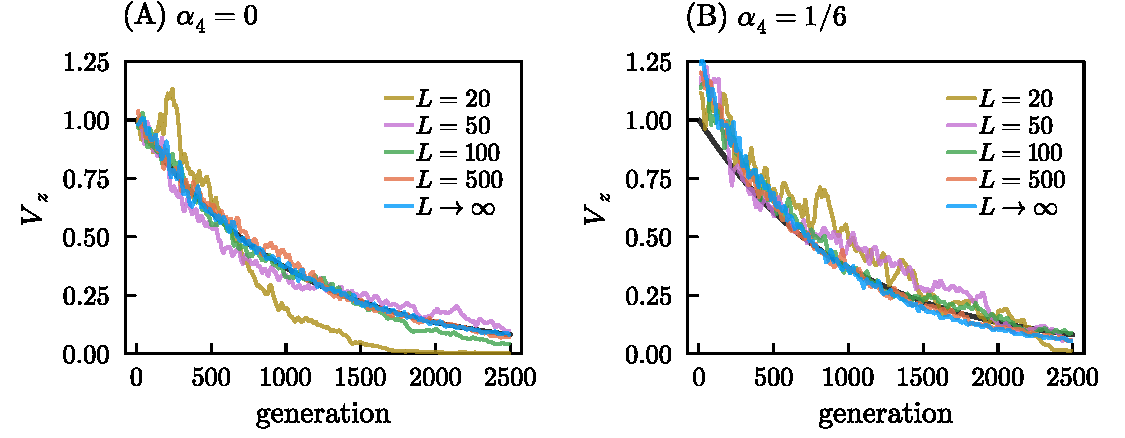
\includegraphics[width=0.9\linewidth]{/home/arthur_z/dev/InfGenetics/doc/img/tetfininf.pdf}
\caption{
The infinitesimal model in autotetraploids.
Comparisons are shown for the decay of the genetic variance ($V_z$) due to
inbreeding in exact simulations of the infinitesimal model in autotetraploids
against individual-based simulations of autotetraploid populations with $L$
unlinked additive loci determining the quantitative trait. 
(A) Simulations of a model without double reduction ($\alpha_4=0$).
(B) Simulations of a model with maximal double reduction ($\alpha_4=1/6$) (for
all loci in the finite $L$ simulations).
We show window-smoothed values for visual clarity, with observed genetic
variances averaged in windows of 20 generations every 10 generations.
The black line marks $e^{-t/4N}$. 
We assume $N=250$ and $V_z(0) = 1$.
\label{fig:vztet}}
\end{figure}


\subsection*{Establishment from a single individual}

Having established the validity of the mixed-ploidy infinitesimal model, we now
use it to study the establishment of polyploids in a marginal habitat to which
migrants from a mixed-ploidy source population are maladapted.

We first consider the establishment of a population from a single migrant
individual with trait value $z_0 = 0$.
We assume $u=0$ and compare the probability of establishment when the migrant
is diploid vs. tetraploid (\cref{fig:est1}).
As noted by \cite{barton2018}, the establishment probability depends
essentially on two dimensionless parameters, $\gamma\sqrt{2V}$ and
$\theta/\sqrt{2V}$, corresponding to the intensity of selection and the degree of
maladaptation, respectively.
We shall scale our results accordingly, assuming $2V=1$ throughout.

We find that reduced inbreeding in tetraploids substantially increases the
establishment probability.
Indeed, in the case where allelic effects are scaled so as to yield the same
equilibrium genetic variance ($\beta = \sqrt{1/2}$), the establishment probability 
for tetraploids can be almost five times as high as in diploids depending on
the selection gradient (\cref{fig:est1}A).
While the probability of establishment becomes lower as the strength of
selection becomes large, the establishment probability does not decrease
monotonically with $\gamma$, i.e. as selection becomes very weak, the
establishment probability also lowers.
This happens because, although the probability of surviving the first couple of
generations becomes higher for weaker selection, adaptation will be slower, and
the risk that genetic variation is exhausted due to inbreeding before the
population is able to reach a consistently positive growth rate is increased.

As expected, the scaling of the equilibrium genetic variance has a profound
effect on the establishment probability, but only when $\beta$ is close to 0.5
(i.e. individual alleles have almost half the effect size in tetraploids
compared to diploids) is the benefit of the slower rate of inbreeding in
tetraploids canceled (\cref{fig:est1}B).


\begin{figure}[t]
\centering
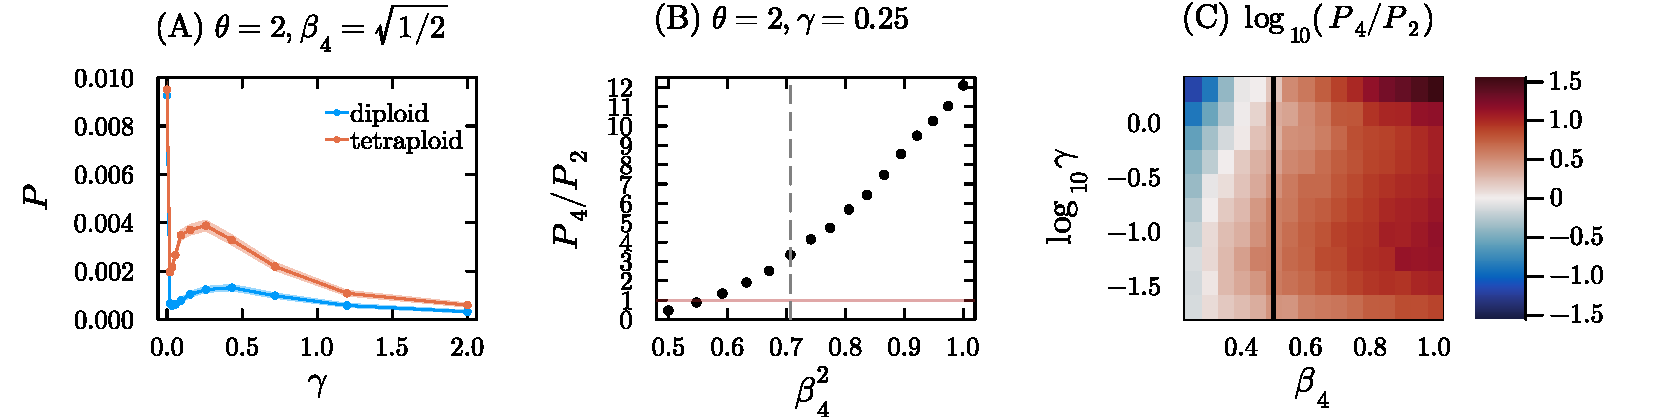
\includegraphics[width=0.9\linewidth]{/home/arthur_z/dev/InfGenetics/doc/img/est1b.pdf}
\caption{
(A) Probability of establishment from a single diploid or tetraploid individual
with trait value $z=0$ for increasing selection intensity $\gamma$.
We assume $m=0$ and $u=0$, i.e. there is no migration, and no unreduced
gametes are produced. The trait is scaled in tetraploids so as to yield the
same genetic variance at HWLE ($\beta_4 = \sqrt{1/2}$)
(B) Probability of a tetraploid individual with trait value $z = 0$
successfully founding a population ($P_4$), relative to the probability for a
diploid individual with the same trait value ($P_2$).
The vertical dashed line marks $\beta_4=\sqrt{1/2}$, for which the variance at
HWLE is identical between diploids and autotetraploids.
All results are estimated from 500.000 replicate simulations.
\label{fig:est1}}
\end{figure}


\subsection*{Establishment under recurrent migration}

We next consider establishment in the new habitat when there is a continuous
influx of migrants coming from a large diploid-dominated mixed-ploidy source
population at cytotype equilibrium.
In this case, establishment is certain to happen eventually, and we are
interested in the probability that a tetraploid population established before a
diploid one does.

We hypothesized that two counteracting processes affect the probability of
autotetraploid establishment in this case.
On the one hand, increased migration will increase the probability that an
otherwise likely successful tetraploid migrant suffers from MCE in the early
generations while the population size is low, because migrants are likely to be
diploid.
On the other hand, tetraploids are strongly reproductively isolated from
the typical migrant, so that they are less prone to maladaptive swamping.
Hence, conditional on evading MCE, they should be able to adapt to the new
habitat at a rate which is not strongly affected by the migration rate.

\begin{figure}[t]
\centering
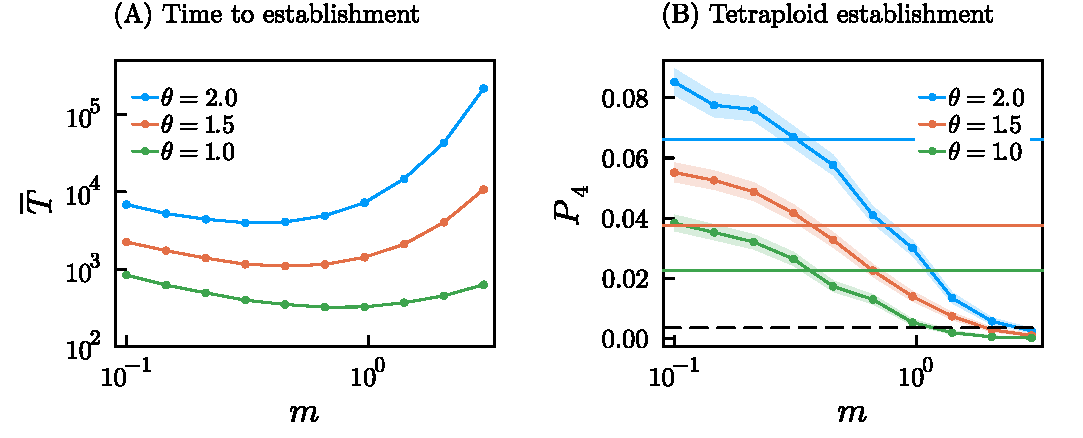
\includegraphics[width=0.9\linewidth]{/home/arthur_z/dev/InfGenetics/doc/img/estwmigration1.pdf}
\caption{
Establishment with recurrent migration.
(A) Expected time until a population is established in the novel habitat for
increasing rates of migration and different degrees of maladaptation
($\bar{z}_s$, the mean trait value in the source population). 
(B) Proportion of simulation replicates in which tetraploids established. 
The shaded area corresponds to Jeffreys' 95\% interval.
The horizontal dashed line marks the proportion of tetraploid migrants (i.e.
the proportion of tetraploids at equilibrium in the source population).
All results are based on 10.000 replicate simulations.
We assume $\gamma=0.25$ and $u=v=0.05$.
\label{fig:estwmig}}
\end{figure}

\subsection*{Loss of self-incompatibility}


\begin{figure}
\centering
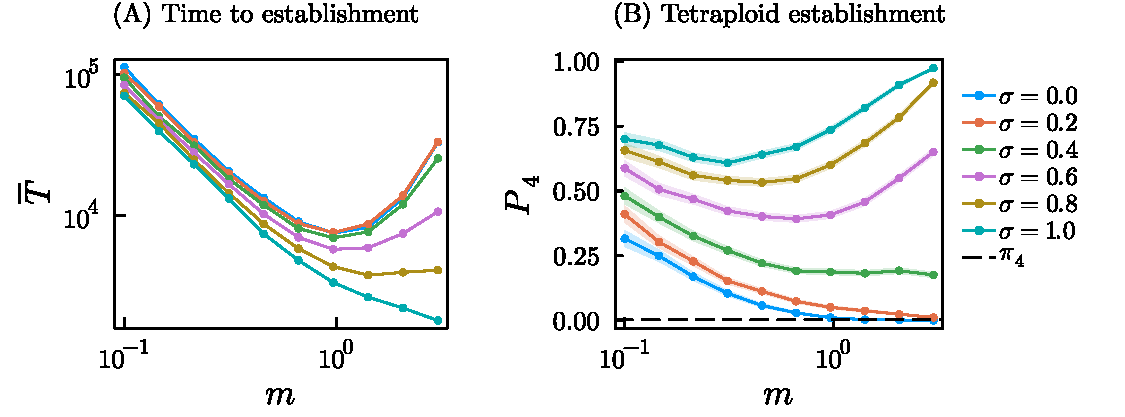
\includegraphics[width=0.9\linewidth]{/home/arthur_z/dev/InfGenetics/doc/img/estwmigration-si.pdf}
\caption{
Establishment with recurrent migration and loss of self-incompatibility in
polyploids.
(A) Expected time until a population is established in the novel habitat for
increasing rates of migration and different self-fertilization rates in
polyploids. Diploids are assumed to be self-incompatible.
Note that $\sigma=0.0$ refers to random self-fertilization (i.e.
self-fertilization with probability $1/N$). 
(B) Proportion of simulation replicates in which tetraploids established. 
The shaded area corresponds to Jeffreys' 95\% interval.
All results are based on 10.000 replicate simulations.
We assume $\gamma=0.25$ and $u=v=0.05$.
\label{fig:}}
\end{figure}


\subsection*{Assortative mating}

\begin{figure}
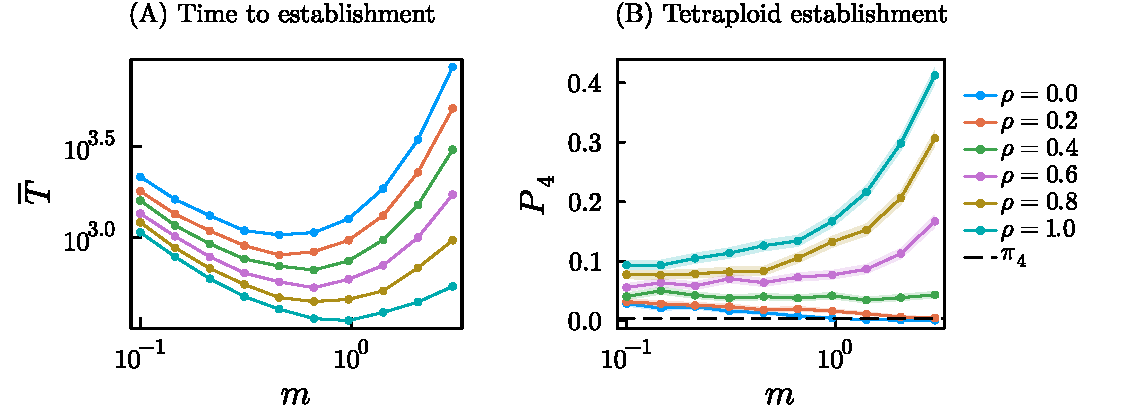
\includegraphics[width=\linewidth]{/home/arthur_z/dev/InfGenetics/doc/img/estwmigration-am.pdf}
\caption{
\label{fig:}}
\end{figure}

\section*{Discussion}


\bibliographystyle{abbrvnat}
\bibliography{/home/arthur_z/vimwiki/bib.bib}
\end{document}
